\documentclass[10pt]{article}         %% What type of document you're writing.
\usepackage{graphicx}
\usepackage{hyperref}
\usepackage[dvipsnames]{xcolor}

%%%%% Preamble

%% Packages to use

\usepackage{amsmath,amsfonts,amssymb}   %% AMS mathematics macros

%% Title Information.

\title{Amazon Data Model}
\author{Leonardo Martinez}
%% \date{29 sep 2020}           %% By default, LaTeX uses the current date

%%%%% The Document

\begin{document}

\maketitle

\begin{abstract}
This document implements the Amazon Data Model.
\end{abstract}

\section{Data Model Desciption}


\textcolor{red}{Proveedores} de Amazon ( \textcolor{green}{codigo, nombre, rating} )\\

\textcolor{red}{Productos} ( \textcolor{green}{codigo, nombre, descripcion, precio, diasentrega, categoria,empresa de reparto} )
\\
\textcolor{red}{Clientes}( \textcolor{green}{ codigo, usuario, password, nombre, direccion} )\\

Los clientes \textcolor{yellow}{compran} n producto

Los proveedores \textcolor{yellow}{surten} n productos


Amazon ...
\section{E-R Model}
\begin{figure}[h]
     \includegraphics[scale=0.4]{amazon_er.png}
     \caption{Amazon E-R Model}
\end{figure}

\section{Relation Model}
\begin{figure}[h]
     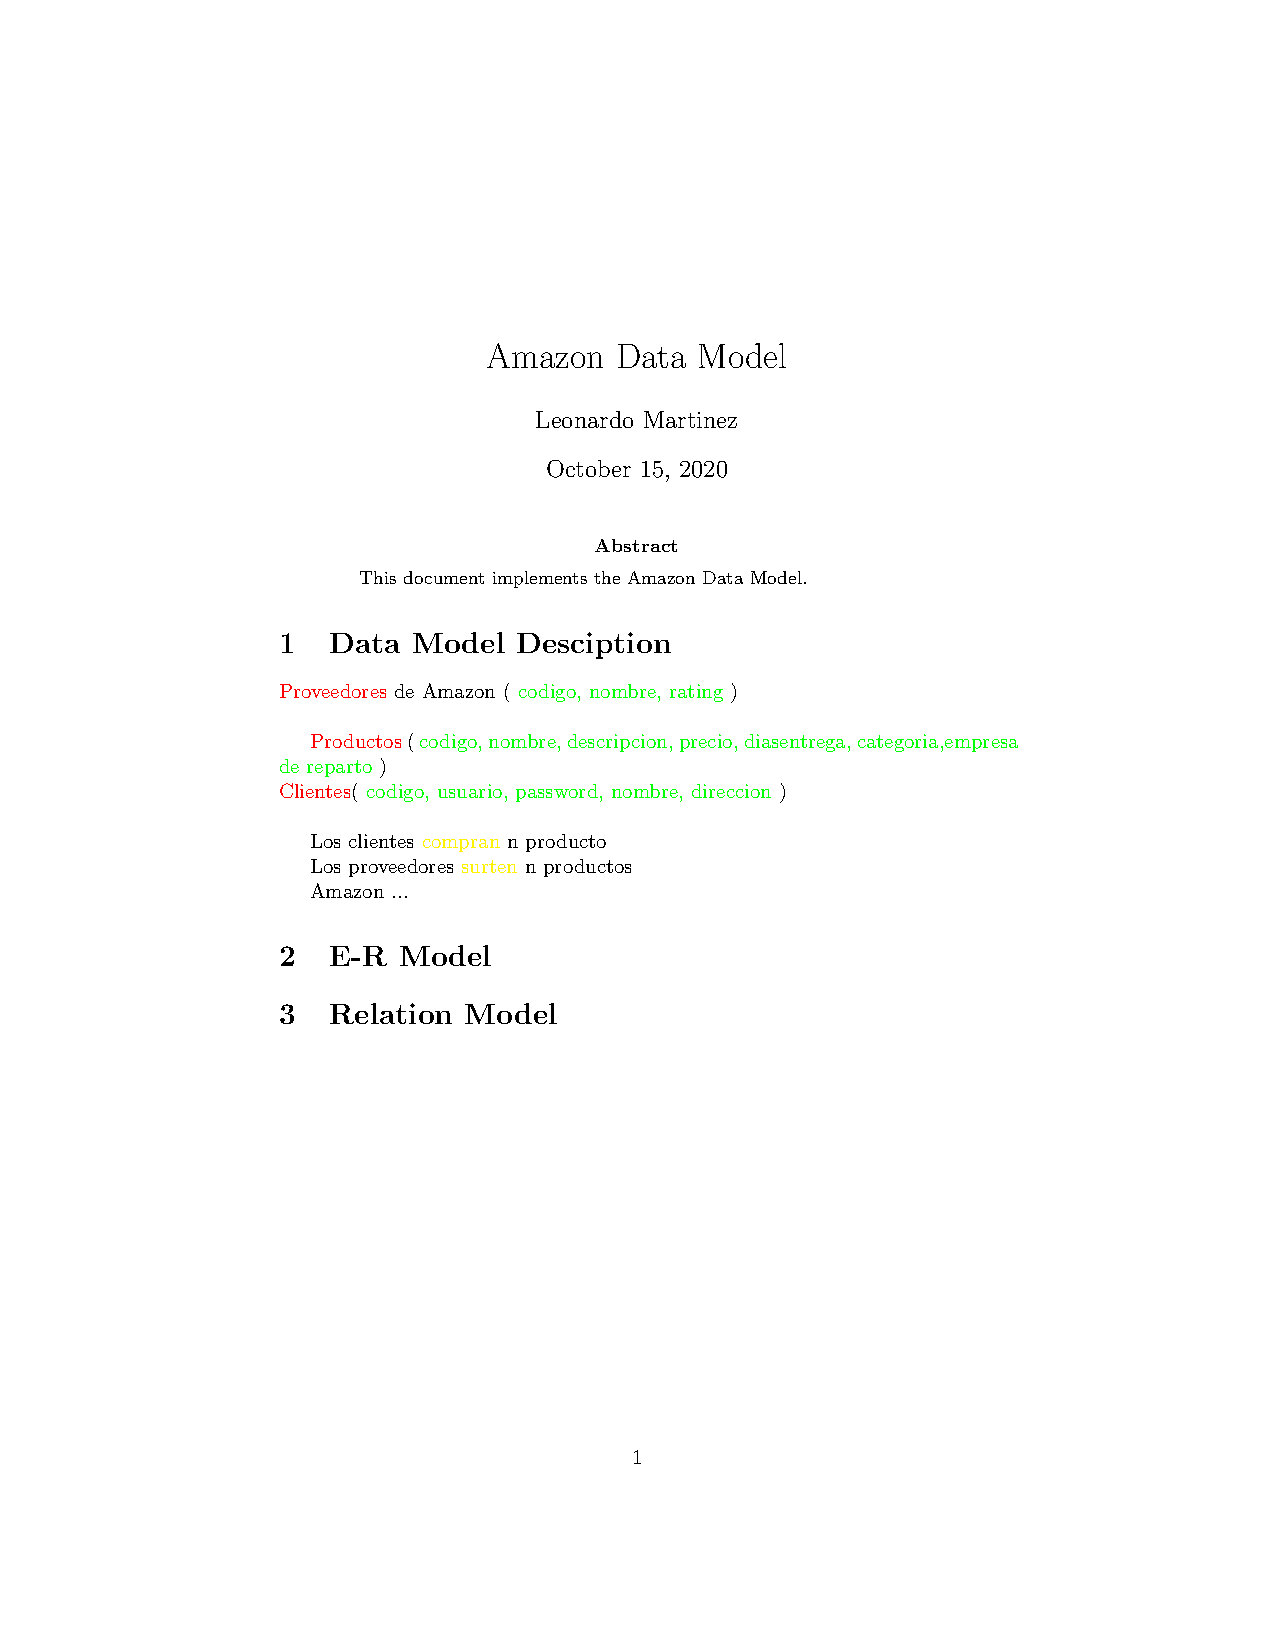
\includegraphics[scale=0.4]{amazon_relation_model.png}
     \caption{Amazon Relation Model}
\end{figure}

\end{document}
